\subsection{Bidirectional forwarding}

In accordance with the recommendations of RFC~8219~\cite{RFC8219}, which -- although focused on IPv6 transition technologies -- 
also defines general benchmarking principles, the same test scenarios were executed under bidirectional traffic conditions.  
This configuration reflects a more realistic networking environment where traffic flows simultaneously in both directions, such as in point-to-point communications,
a VPN tunnels, or client-server interactions involving both requests and responses.  
Unlike the one-way setup, bidirectional forwarding places a greater strain on system resources by utilizing both receive (RX) and transmit (TX) paths concurrently, 
which may reveal bottlenecks or limitations not evident in unidirectional traffic scenarios.
It is important to note that bidirectional tests generate traffic at a rate of \textit{X}\,Gbit/s in each direction, resulting in a total system load of \textit{2X}\,Gbit/s.

%----------------------------------
\subsubsection{1 Gbps Test Results}

As shown in Table~\ref{tab:bidirectional-1g}, bidirectional forwarding at 1\,Gbit/s resulted in increased latency across all VPP configurations compared to unidirectional traffic. 
VPP-4 and VPP-10 achieved latency levels similar to those observed in the 10\,Gbit/s unidirectional test, except for the 64-byte frame case, which remained closer to the 1\,Gbit/s results.
Notably, VPP-1 performed significantly worse than in the unidirectional scenario, showing latency figures comparable to those seen in the 25\,Gbit/s unidirectional test. 
This indicates that polling multiple interfaces negatively impacts latency performance in VPP.
While VPP also polled both interfaces in the unidirectional tests, the secondary interface had no traffic, and was merely checked periodically. 
In the bidirectional case, however, VPP had to process packet vectors from both NICs, which clearly introduced additional latency. 
Since VPP processes packets in vectors from one interface at a time, traffic arriving on the second interface must wait until the current batch is completed. 
This serial processing model contributes to increased latency under bidirectional load.
Interestingly, the Linux network stack outperformed all VPP configurations when average or large frames were used, achieving the lowest latency in these scenarios. 
By comparison, VPP delivered better results in the small frame tests, showcasing its capability to handle high-packet-rate workloads efficiently.

\begin{table}[h!]
\centering
\caption{Results of bidirectional 1~Gbit/s tests}
\begin{tabular}{|c|l|r|r|r|r|}
\hline
\textbf{} & \textbf{Config} & \textbf{Energy [Wh]} & \textbf{Pkt Loss [\%]} & \textbf{Avg Lat [$\mu$s]} & \textbf{Jitter [$\mu$s]} \\
\hline
\multirow{4}{*}{\rotatebox{90}{64B}}    
    & VPP-1  & 5.42 & 0.00 & 27.83 & 10.48 \\
    & VPP-4  & 6.30 & 0.00 & 30.18 & 14.08 \\
    & VPP-10 & 8.00 & 0.00 & 30.45 & 13.48 \\
    & Linux  & 7.20 & 0.00 & 147.68 & 100.05 \\
\hline
\multirow{4}{*}{\rotatebox{90}{512B}}   
    & VPP-1  & 5.80 & 0.00 & 28.05 & 15.70 \\
    & VPP-4  & 6.45 & 0.00 & 26.73 & 17.30 \\
    & VPP-10 & 7.93 & 0.00 & 24.56 & 16.30 \\
    & Linux  & 6.35 & 0.00 & 39.83 & 39.20 \\
\hline
\multirow{4}{*}{\rotatebox{90}{889B}}   
    & VPP-1  & 5.66 & 0.00 & 26.10 & 14.50 \\
    & VPP-4  & 6.43 & 0.00 & 26.13 & 17.53 \\
    & VPP-10 & 7.78 & 0.00 & 26.28 & 17.00 \\
    & Linux  & 6.27 & 0.00 & 17.4  & 12.38 \\
\hline
\multirow{4}{*}{\rotatebox{90}{1280B}}  
    & VPP-1  & 5.75 & 0.00 & 25.20 & 12.45 \\
    & VPP-4  & 6.39 & 0.00 & 25.23 & 17.10 \\
    & VPP-10 & 7.85 & 0.00 & 27.40 & 18.33 \\
    & Linux  & 6.21 & 0.00 & 12.68 & 7.28  \\
\hline
\multirow{4}{*}{\rotatebox{90}{1518B}}  
    & VPP-1  & 5.77 & 0.00 & 25.10 & 13.15 \\
    & VPP-4  & 6.36 & 0.00 & 25.53 & 15.63 \\
    & VPP-10 & TODO?&      &       &       \\
    & Linux  & 6.13 & 0.00 & 12.40  & 9.40  \\
\hline
\end{tabular}
\label{tab:bidirectional-1g}
\end{table}

Figure~\ref{fig:bi-1g} shows that the results for PPWh and BPWh are similar to those of the one-way 1\,Gbit/s test, 
although Linux exhibits slightly lower efficiency compared to VPP then was observed in one-way scenario.



\begin{figure}[!htbp]
    \centering
    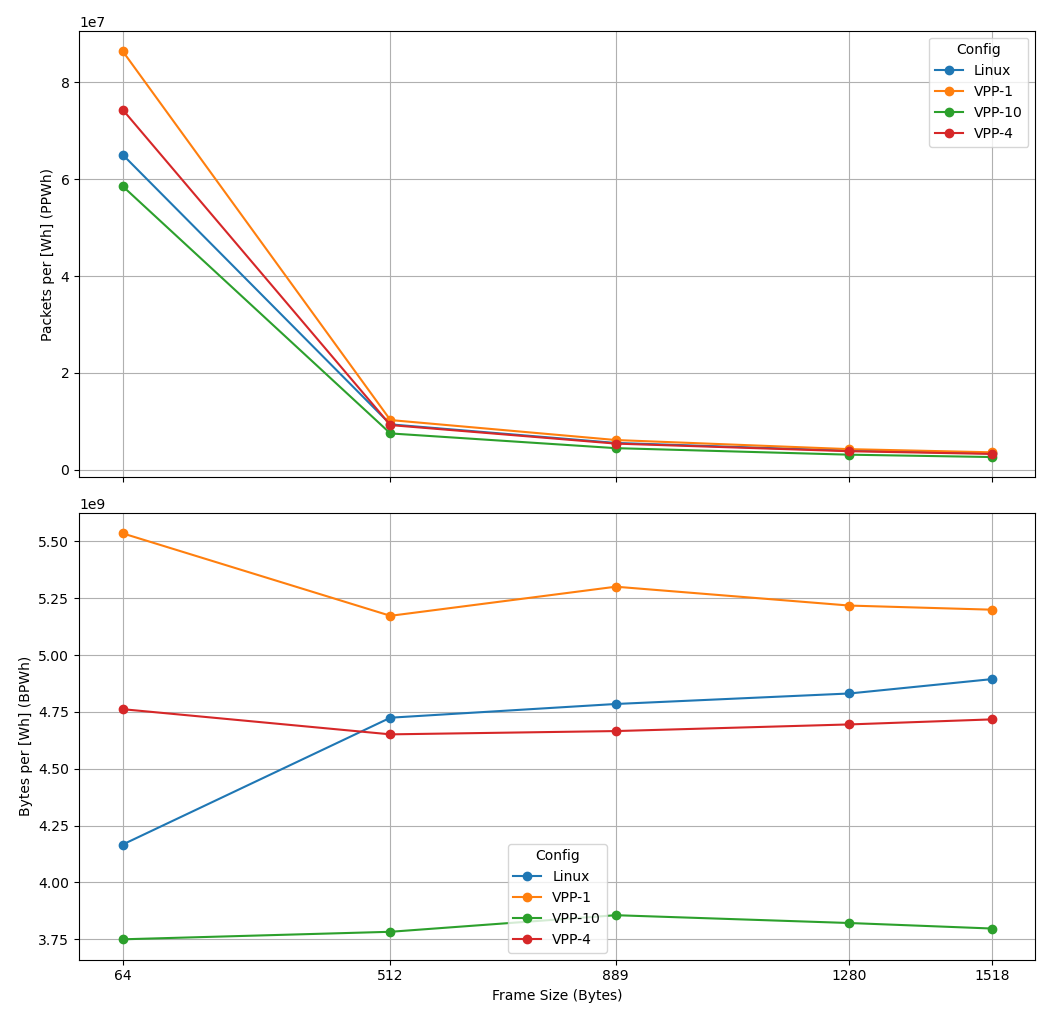
\includegraphics[width=\linewidth]{images/consumption-bi-1g.png}
    \caption{Energy efficiency per delivered data in bidirectional 1\,Gbit/s.}
    \label{fig:bi-1g}
\end{figure}

%-----------------------------------
%-----------------------------------
%-----------------------------------
\subsubsection{10 Gbps Test Results}

The results of the 10\,Gbit/s bidirectional test, presented in Table~\ref{tab:bidirectional-10g}, are more comparable to the 25\,Gbit/s one-way test than to the 10\,Gbit/s one-way scenario, 
indicating that serving an additional NIC had no negative impact on performance.  
The only notable difference is that the VPP-1 configuration achieved better latency in one-way 25\,Gbit/s forwarding for medium and large frames, despite handling a higher total traffic load.  
In the bidirectional test, with a total throughput of 20\,Gbit/s, all VPP configurations -- except in the 64-byte frame scenario -- 
were able to handle the traffic successfully while maintaining stable latency.  
By contrast, the Linux stack struggled to process the full traffic load. Even in cases where it managed to deliver all packets (i.e., with larger frames), it still exhibited significantly higher latency.

\begin{table}[h!]
\centering
\caption{Results of bidirectional 10~Gbit/s tests}
\begin{tabular}{|c|l|r|r|r|r|}
\hline
\textbf{} & \textbf{Config} & \textbf{Energy [Wh]} & \textbf{Pkt Loss [\%]} & \textbf{Avg Lat [$\mu$s]} & \textbf{Jitter [$\mu$s]} \\
\hline
\multirow{4}{*}{\rotatebox{90}{64B}}    
    & VPP-1  & 5.52 & 70.40 & 537.43 & 12.15 \\
    & VPP-4  & 6.51 & 30.47 & 188.40 & 7.23  \\
    & VPP-10 & 8.40 & 0.00  & 42.05  & 12.55 \\
    & Linux  & 7.24 & 92.91 & 8408.15 & 924.05 \\
\hline
\multirow{4}{*}{\rotatebox{90}{512B}}   
    & VPP-1  & 5.80 & 0.00 & 27.75 & 11.73 \\
    & VPP-4  & 6.55 & 0.00 & 32.50 & 14.48 \\
    & VPP-10 & 7.99 & 0.00 & 30.58 & 15.38 \\
    & Linux  & 7.44 & 25.22 & 3837.13 & 172.03 \\
\hline
\multirow{4}{*}{\rotatebox{90}{889B}}   
    & VPP-1  & 5.77 & 0.00 & 34.00 & 15.15 \\
    & VPP-4  & 6.55 & 0.00 & 32.50 & 14.48 \\
    & VPP-10 & 7.98 & 0.00 & 30.50 & 16.35 \\
    & Linux  & 7.19 & 0.00 & 110.20 & 82   \\
\hline
\multirow{4}{*}{\rotatebox{90}{1280B}}  
    & VPP-1  & 5.81 & 0.00 & 34.15 & 14.86 \\
    & VPP-4  & 6.37 & 0.00 & 32.73 & 16.88 \\
    & VPP-10 & 8.01 & 0.00 & 32.20 & 15.85 \\
    & Linux  & 6.97 & 0.00 & 77.45 & 70.33 \\
\hline
\multirow{4}{*}{\rotatebox{90}{1518B}}  
    & VPP-1  & 5.78 & 0.00 & 33.80 & 16.10 \\
    & VPP-4  & 6.36 & 0.00 & 25.56 & 15.63 \\
    & VPP-10 & 7.85 & 0.00 & 27.40 & 18.33 \\
    & Linux  & 6.89 & 0.00 & 72.78 & 70.08 \\
\hline
\end{tabular}
\label{tab:bidirectional-10g}
\end{table}

The energy efficiency, in terms of BPWh and PPWh, is similar to that observed in the one-way 10\,Gbit/s and 25\,Gbit/s tests, with results being more closely aligned with the 25\,Gbit/s case.  
Given the combined throughput of 20\,Gbit/s, this behavior was expected.  
The corresponding results are visualized in Figure~\ref{fig:bi-10g}.

\begin{figure}[!htbp]
    \centering
    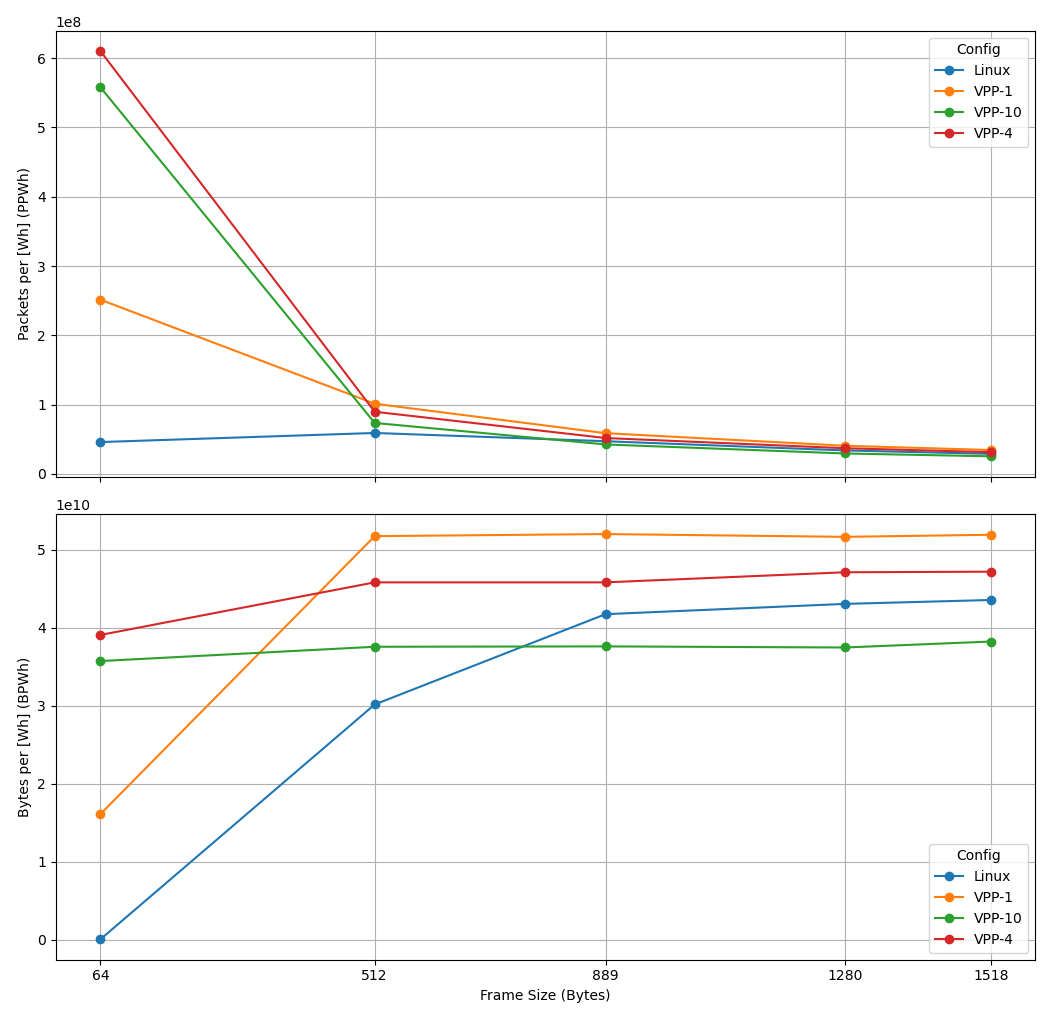
\includegraphics[width=\linewidth]{images/consumption-bi-10g.png}
    \caption{Energy efficiency per delivered data in bidirectional 10\,Gbit/s.}
    \label{fig:bi-10g}
\end{figure}

%-----------------------------------
%-----------------------------------
%-----------------------------------
\subsubsection{25 Gbps Test Results}

As with the previous test, the results presented in Table~\ref{tab:bidirectional-25g} more closely resemble those of the one-way 40\,Gbit/s scenario.  
Since Linux was unable to deliver all packets in that test, it is not surprising that even more packets were dropped in this case.  
Interestingly, in all VPP configurations where packet loss occurred, the percentage of dropped packets was slightly lower compared to the one-way 40\,Gbit/s test, 
despite the higher total throughput of 50\,Gbi/s.  
One possible explanation is that bidirectional forwarding leads to more balanced utilization of RX queues across multiple cores.  
Moreover, in scenarios without packet loss, VPP maintained stable latency values -- although increased compared to the previous 10\,Gbit/s bidirectional experiment.

\begin{table}[h!]
\centering
\caption{Results of bidirectional 25~Gbit/s tests}
\begin{tabular}{|c|l|r|r|r|r|}
\hline
\textbf{} & \textbf{Config} & \textbf{Energy [Wh]} & \textbf{Pkt Loss [\%]} & \textbf{Avg Lat [$\mu$s]} & \textbf{Jitter [$\mu$s]} \\
\hline
\multirow{4}{*}{\rotatebox{90}{64B}}    
    & VPP-1  & 5.54 & 88.16 & 545.50 & 12.30 \\
    & VPP-4  & 6.60 & 64.58 & 185.08 & 8.18  \\
    & VPP-10 & 8.40 & 42.05 & 159.55 & 12.55 \\
    & Linux  & 7.23 & 97.09 & 9266.88 & 1409.90 \\
\hline
\multirow{4}{*}{\rotatebox{90}{512B}}   
    & VPP-1  & 5.80 & 28.95 & 294.13 & 25.80 \\
    & VPP-4  & 6.72 & 0.00  & 38.18  & 13.28 \\
    & VPP-10 & 8.20 & 0.00  & 37.38  & 15.43 \\
    & Linux  & 7.53 & 76.86 & 8079.28 & 644.00 \\
\hline
\multirow{4}{*}{\rotatebox{90}{889B}}   
    & VPP-1  & 5.82 & 0.01  & 43.63 & 17.15 \\
    & VPP-4  & 6.71 & 0.00  & 39.58  & 16.38 \\
    & VPP-10 & 8.16 & 0.00  & 36.83  & 16.65 \\
    & Linux  & 7.50 & 57.50 & 16506.75 & 814.28 \\
\hline
\multirow{4}{*}{\rotatebox{90}{1280B}}  
    & VPP-1  & 5.86 & 0.00  & 40.40  & 15.73 \\
    & VPP-4  & 6.63 & 0.00  & 39.43  & 15.55 \\
    & VPP-10 & 8.22 & 0.00  & 37.93  & 15.25 \\
    & Linux  & 7.50 & 32.67 & 13791.63 & 357.95 \\
\hline
\multirow{4}{*}{\rotatebox{90}{1518B}}  
    & VPP-1  & 5.84 & 0.00  & 43.95  & 18.58 \\
    & VPP-4  & 6.65 & 0.00  & 38.38  & 15.88 \\
    & VPP-10 & 8.17 & 0.00  & 36.28  & 17.78 \\
    & Linux  & 7.70 & 10.57 & 6568.30 & 112.68 \\
\hline
\end{tabular}
\label{tab:bidirectional-25g}
\end{table}

Concerning energy efficiency, it is worth noting that the Linux network stack remained the least energy-efficient across all frame sizes, primarily due to the high packet loss.  
The results closely resemble those observed in the one-way 40\,Gbit/s test.  
A graph visualizing these results is shown in Figure~\ref{fig:bi-25g}.

\begin{figure}[!htbp]
    \centering
    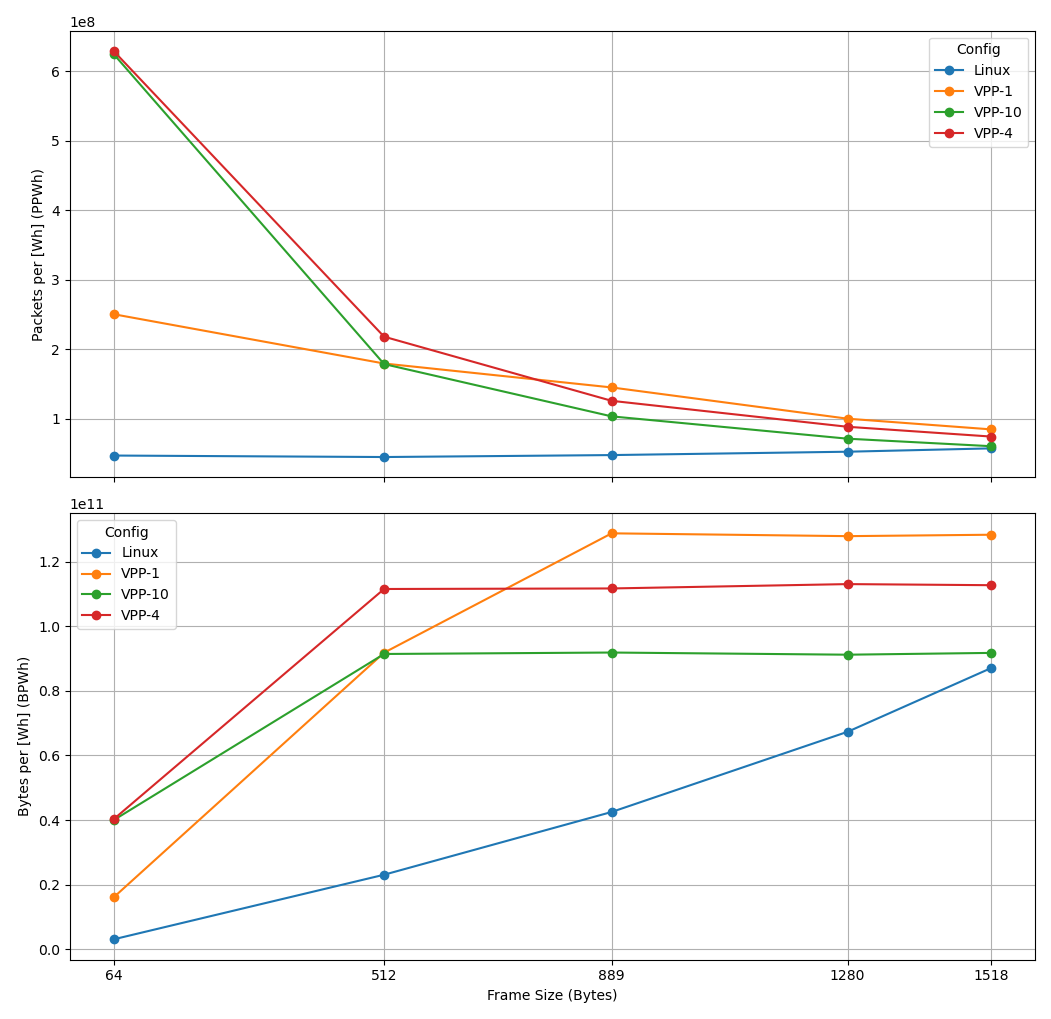
\includegraphics[width=\linewidth]{images/consumption-bi-25g.png}
    \caption{Energy efficiency per delivered data in bidirectional 25\,Gbit/s.}
    \label{fig:bi-25g}
\end{figure}



%-----------------------------------
%-----------------------------------
%-----------------------------------
\subsubsection{40 Gbps Test Results}

This final and most demanding test, with a total bidirectional throughput of 80\,Gbit/s, clearly demonstrates the scalability of VPP compared to the Linux network stack.  
In every frame size scenario, Linux dropped more than half of all packets, confirming its limited capability to handle high-throughput workloads.  
VPP, on the other hand, managed to process a substantial portion of the traffic even in the smallest frame sizes, 
and at higher configurations (VPP-4 and VPP-10) was able to eliminate packet loss entirely for medium and large frames.  
These results further underline the advantages of user-space packet processing under extreme conditions.
The results are summarised in Table~\ref{tab:bidirectional-40g}.

\begin{table}[h!]
\centering
\caption{Results of bidirectional 40~Gbit/s tests}
\begin{tabular}{|c|l|r|r|r|r|}
\hline
\textbf{} & \textbf{Config} & \textbf{Energy [Wh]} & \textbf{Pkt Loss [\%]} & \textbf{Avg Lat [$\mu$s]} & \textbf{Jitter [$\mu$s]} \\
\hline
\multirow{4}{*}{\rotatebox{90}{64B}}    
    & VPP-1  & 5.52 & 92.60 & 543.45 & 13.25 \\
    & VPP-4  & 6.64 & 77.42 & 182.70 & 6.58  \\
    & VPP-10 & 8.38 & 71.13 & 156.08 & 10.375 \\
    & Linux  & 7.22 & 98.22 & 9256.2 & 1353.3 \\
\hline
\multirow{4}{*}{\rotatebox{90}{512B}}   
    & VPP-1  & 5.82 & 57.83 & 317.70 & 103.95 \\
    & VPP-4  & 6.74 & 19.06 & 175.25 & 21.63 \\
    & VPP-10 & 8.42 & 13.00 & 168.70 & 20.28 \\
    & Linux  & 7.59 & 86.28 & 8976.75 & 924.63 \\
\hline
\multirow{4}{*}{\rotatebox{90}{889B}}   
    & VPP-1  & 5.84 & 37.21 & 215.45 & 47.30 \\
    & VPP-4  & 6.89 & 1.29  & 142.7  & 17.2 \\
    & VPP-10 & 8.43 & 0.00  & 52.48  & 15.38 \\
    & Linux  & 7.64 & 76.43 & 17567.73 & 1555.53 \\
\hline
\multirow{4}{*}{\rotatebox{90}{1280B}}  
    & VPP-1  & 5.89 & 18.32 & 179.13 & 36.65 \\
    & VPP-4  & 6.86 & 0.00  & 54.68  & 18.28 \\
    & VPP-10 & 8.39 & 0.00  & 49.63  & 17.40 \\
    & Linux  & 7.48 & 64.37 & 16067.48 & 673.3 \\
\hline
\multirow{4}{*}{\rotatebox{90}{1518B}}  
    & VPP-1  & 5.86 & 14.67 & 159.55 & 36.45 \\
    & VPP-4  & 6.86 & 0.00  & 57.20  & 20.43 \\
    & VPP-10 & 8.38 & 0.00  & 51.63  & 19.63 \\
    & Linux  & 7.56 & 54.60 & 12835.1 & 588.1 \\
\hline
\end{tabular}
\label{tab:bidirectional-40g}
\end{table}

As shown in the energy efficiency graph in Figure~\ref{fig:bi-40g}, Linux clearly remains the least energy-efficient configuration.  
Due to high packet loss, the energy efficiency of VPP-1 also declined, falling below that of VPP-4.

\begin{figure}[!htbp]
    \centering
    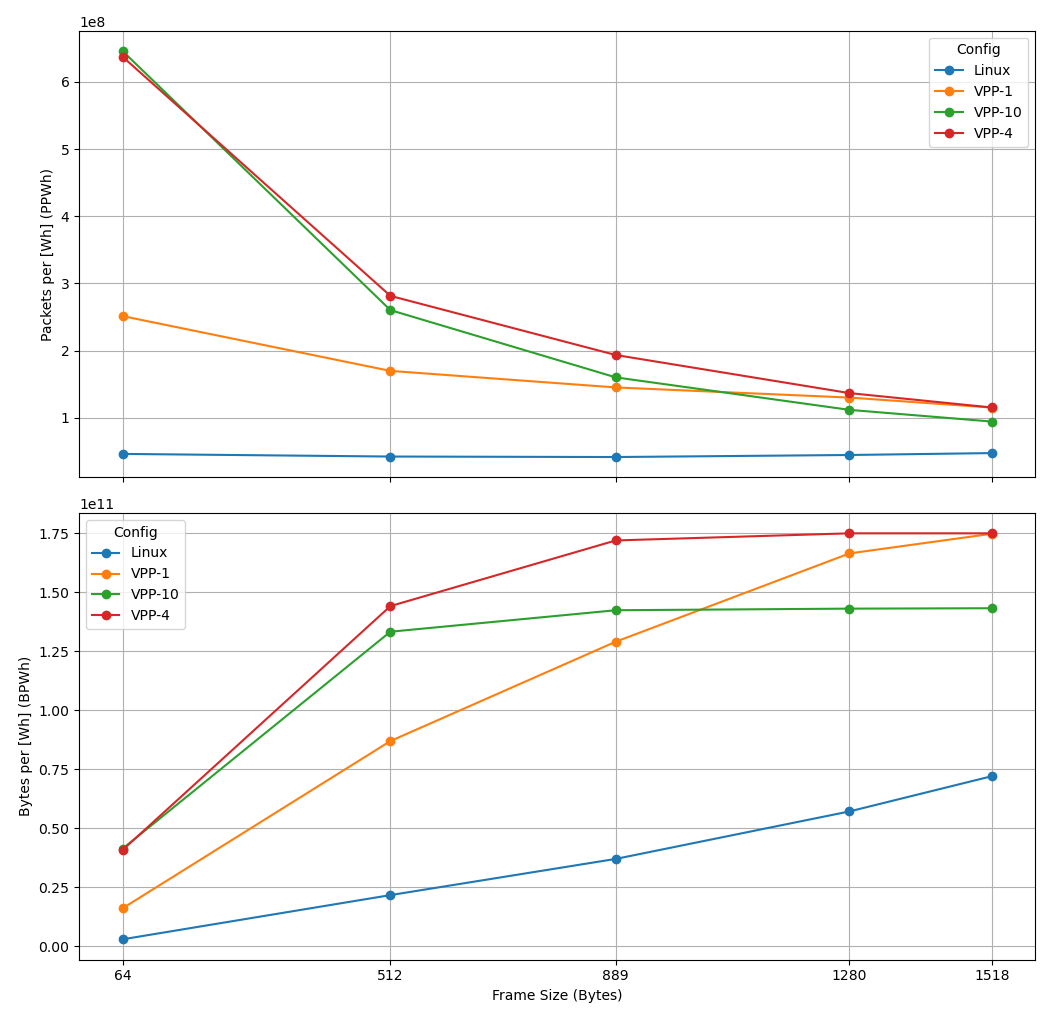
\includegraphics[width=\linewidth]{images/consumption-bi-40g.png}
    \caption{Energy efficiency per delivered data in bidirectional 40\,Gbit/s.}
    \label{fig:bi-40g}
\end{figure}

